\section{Beispiele}
\begin{frame}{Berichte}
    \begin{itemize}
        \item Laborberichte 
    \end{itemize}
    \begin{figure}[htpb]
        \centering
        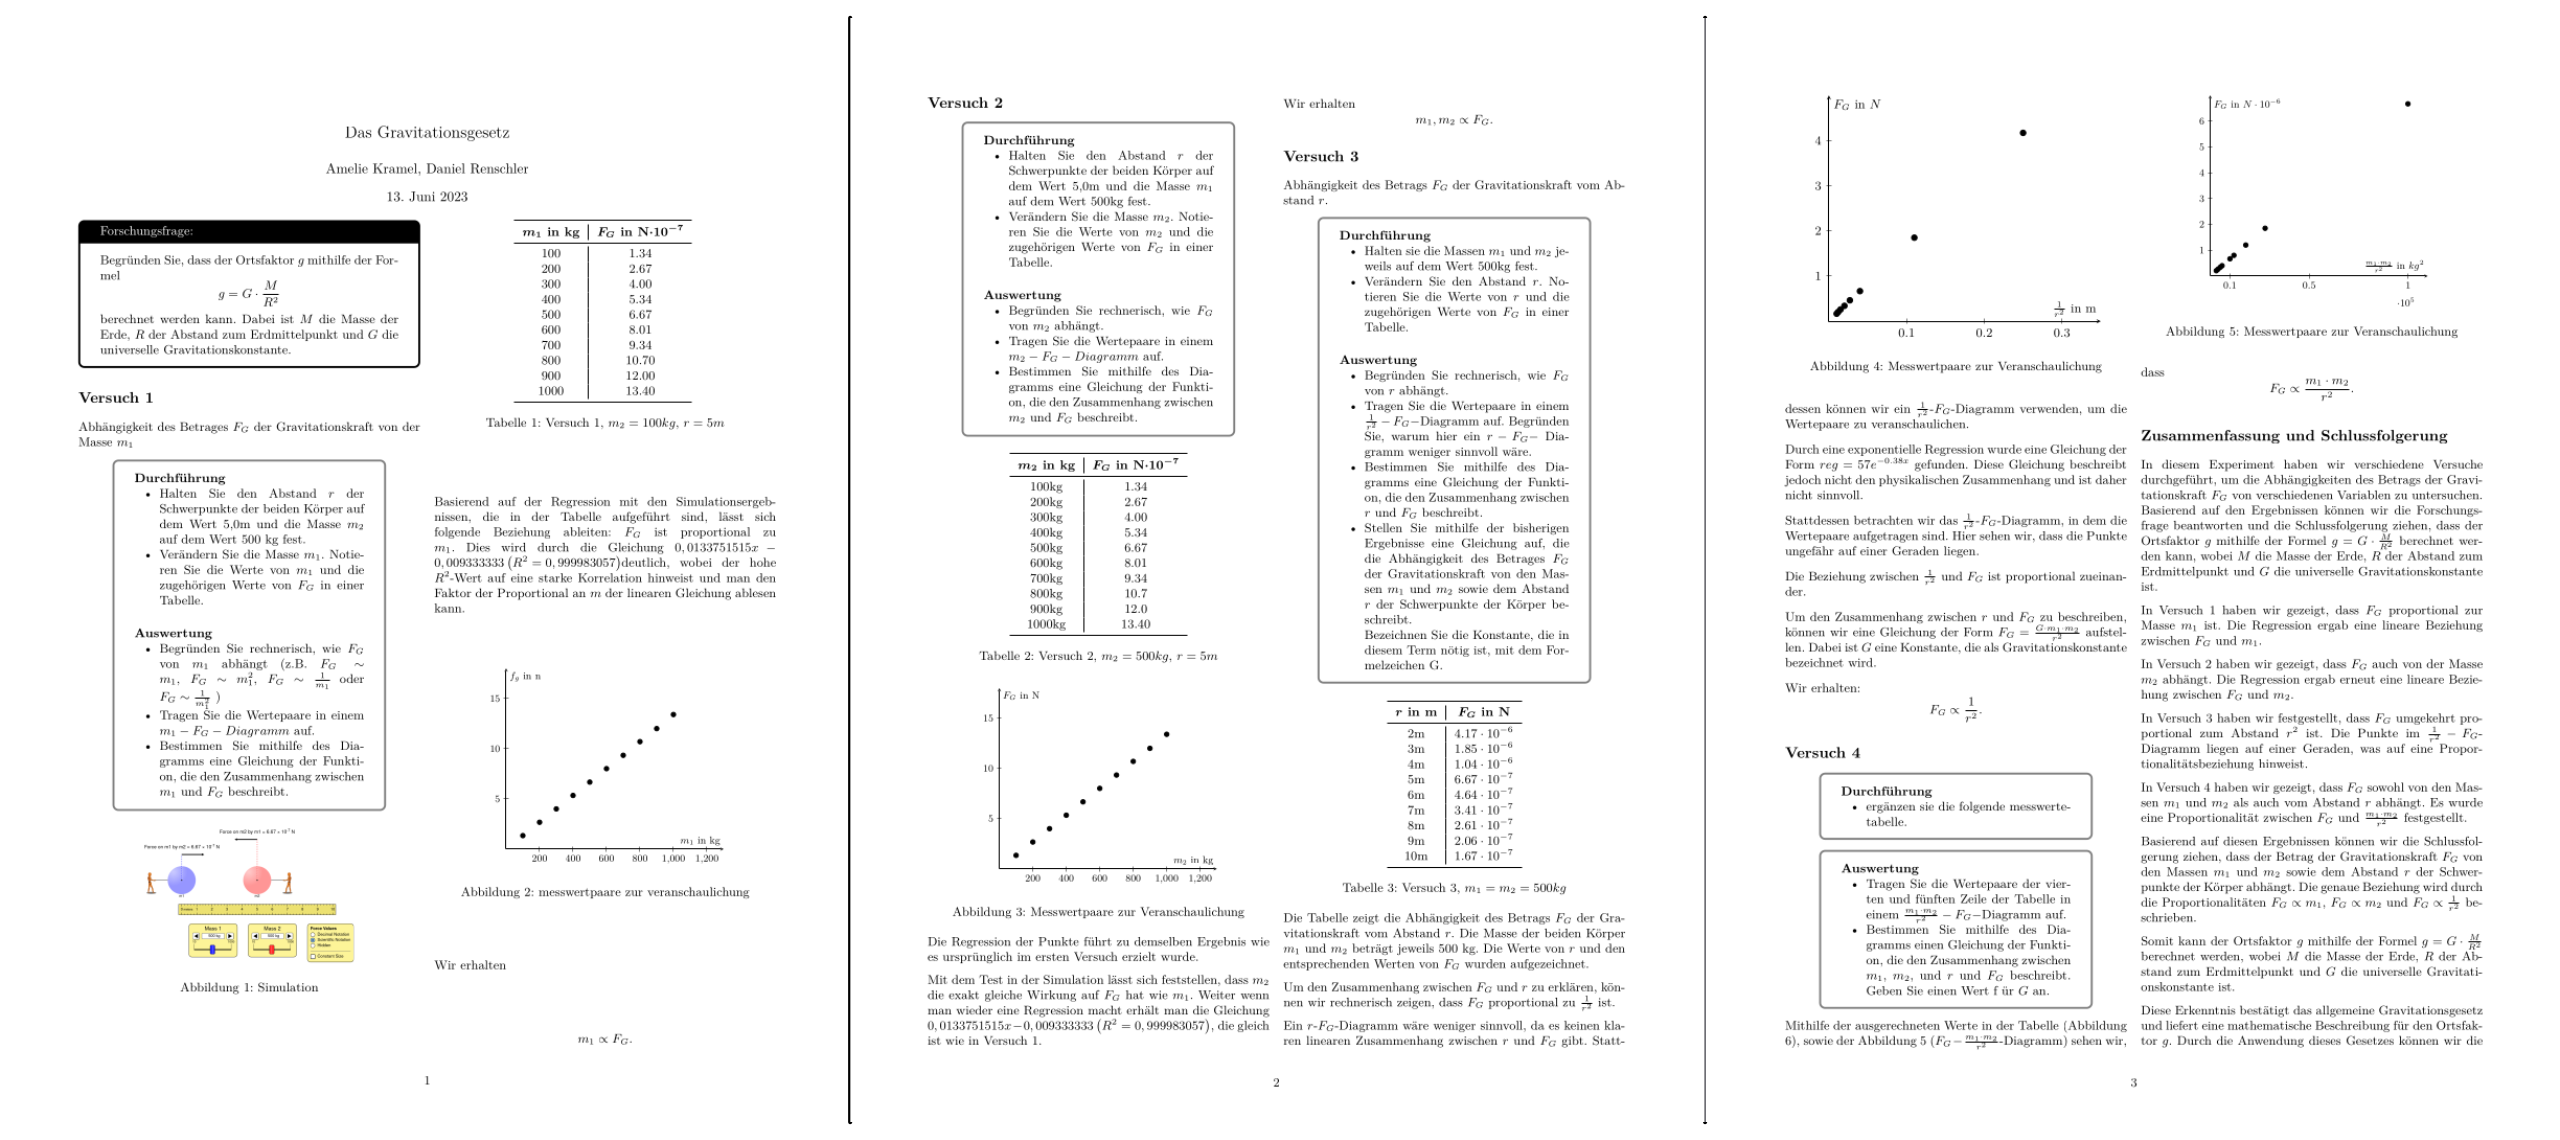
\includegraphics[width=1\textwidth]{./figs/am stueck.png}
        \caption{Laborprotokoll Gravitationsgesetz}
        \label{fig:labor}
    \end{figure}
\end{frame}



\begin{frame}{Paper}
    \begin{figure}[htpb]
        \centering
        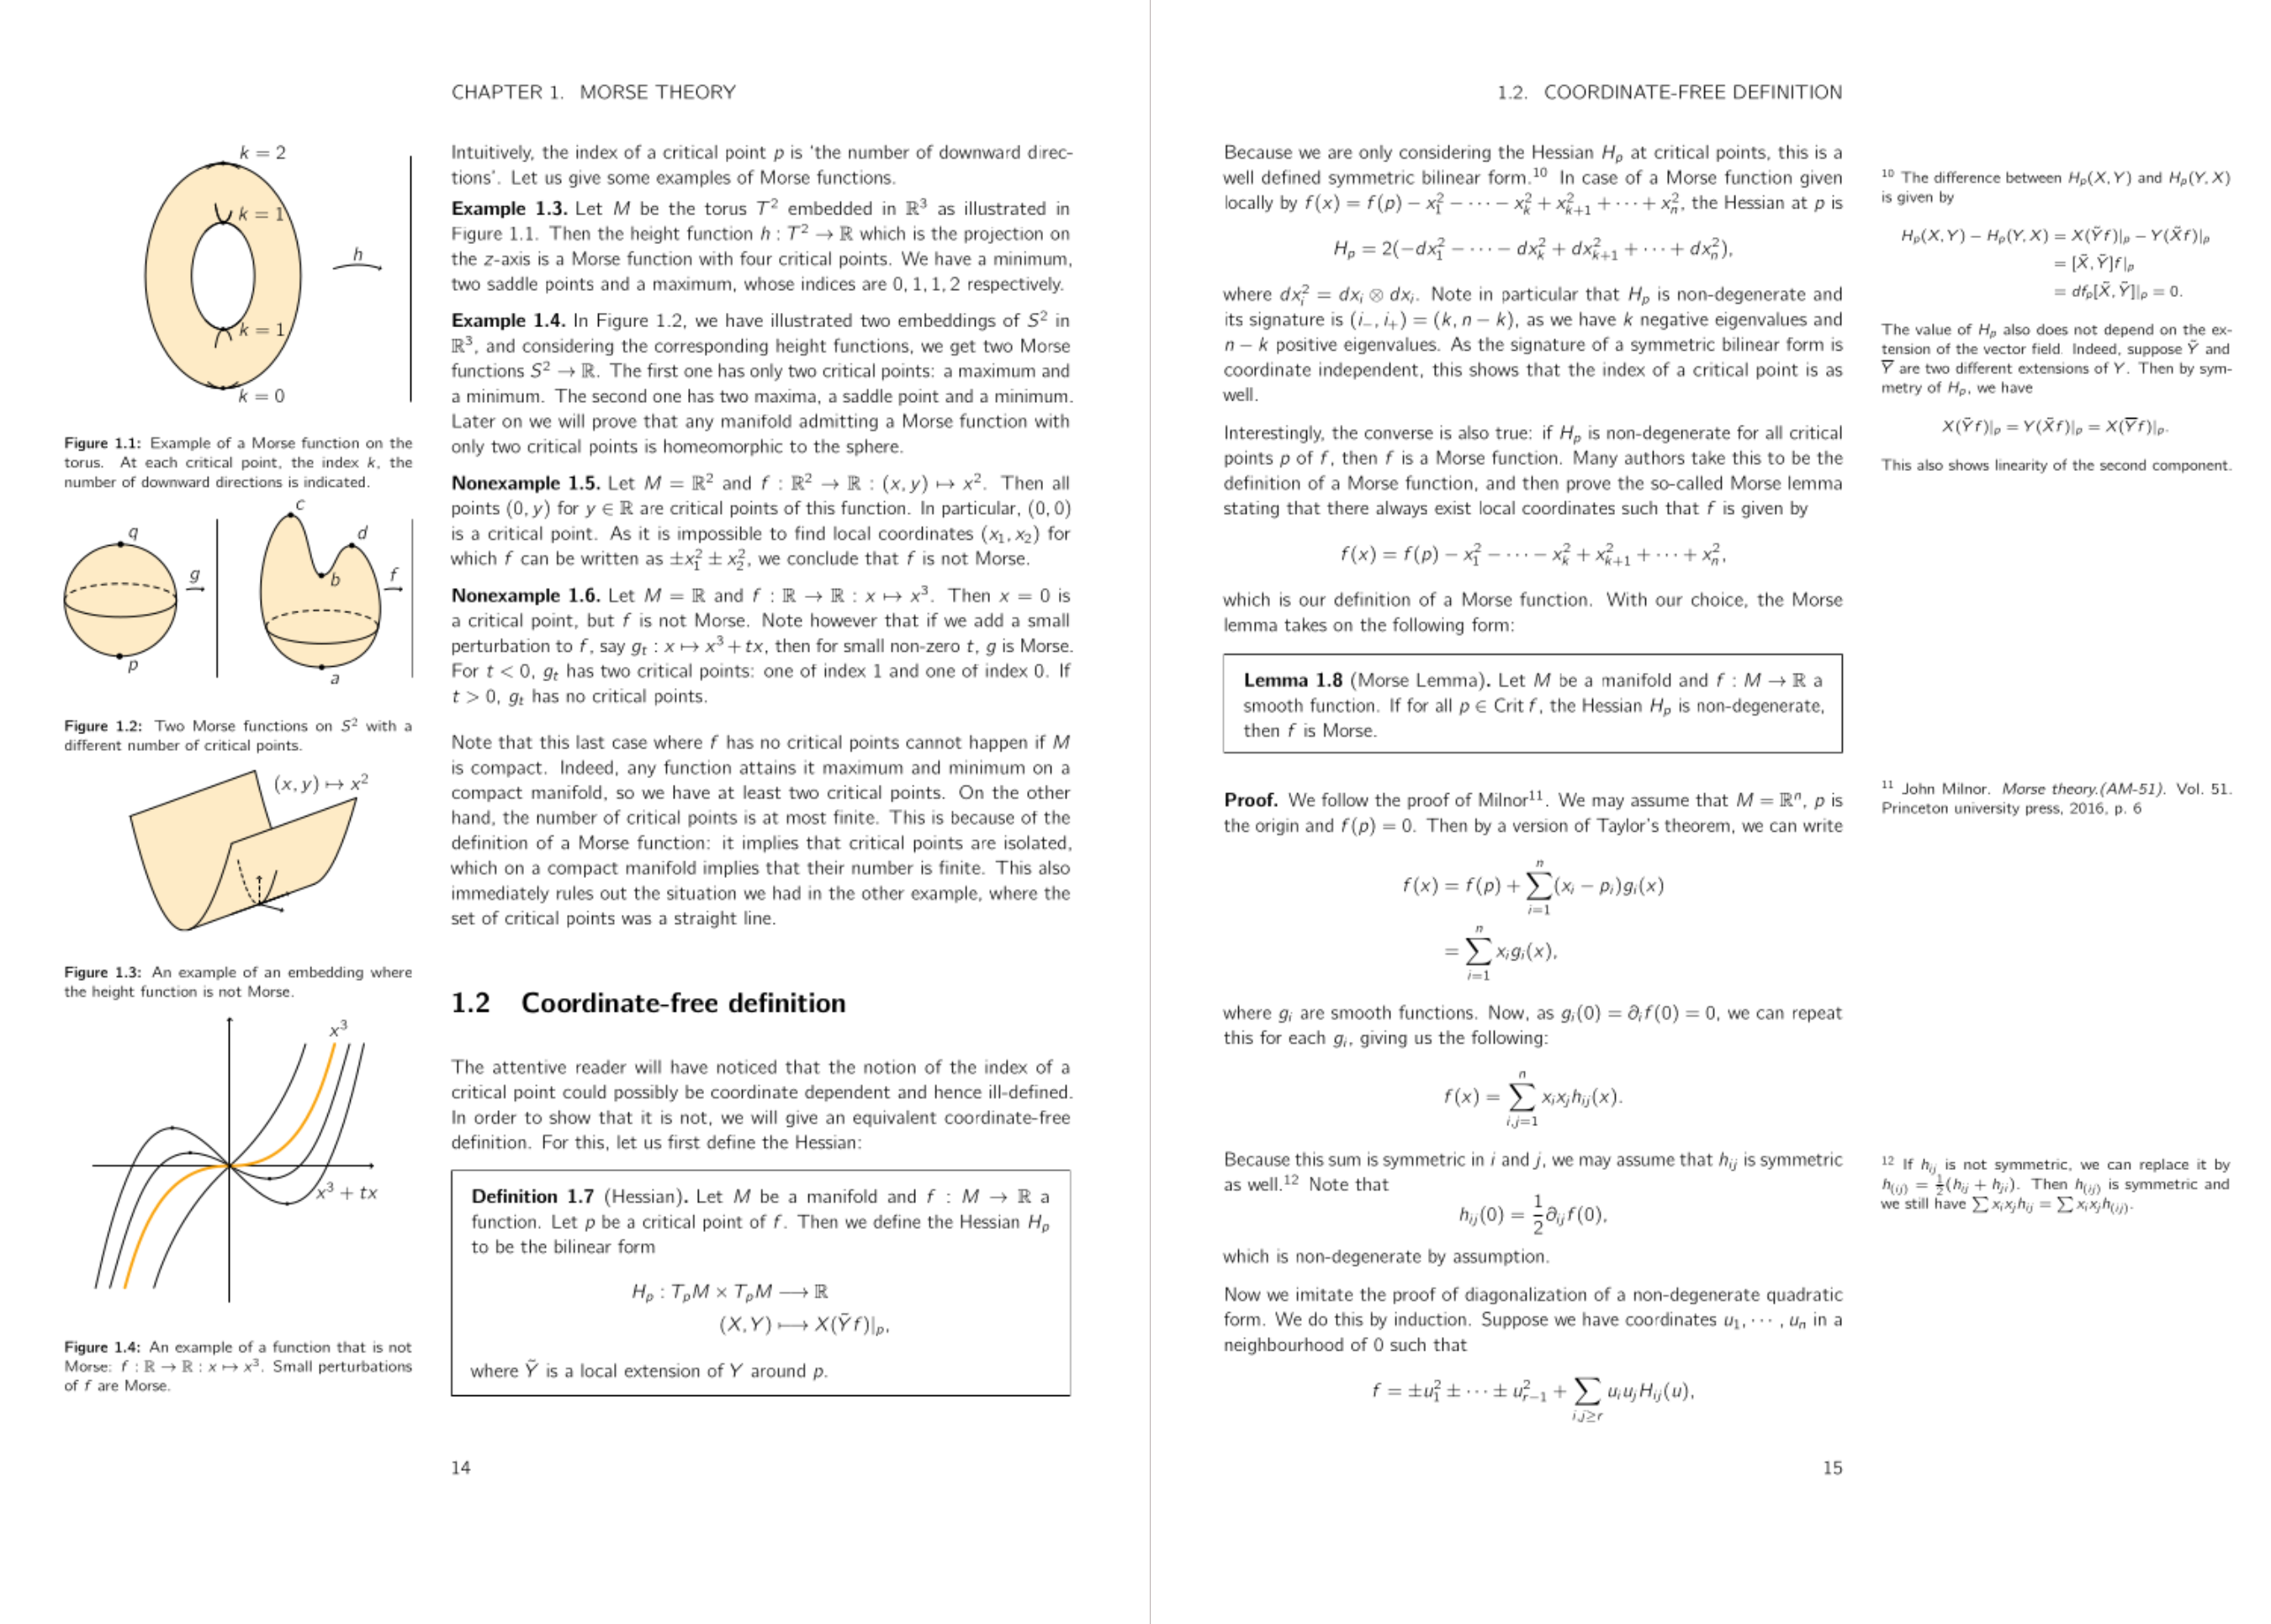
\includegraphics[width=0.7\textwidth]{./figs/example-paper.png}
        \caption{Auszug einer Masterarbeit \"uber Morse Theory}
    \end{figure}
\end{frame}


\begin{frame}{Beispiel 1}


Beispiele:
\begin{itemize}
    \item Irgendwas mit Euler \cite{baranek2023randomized}
        \[ \mathcal{L} = \frac{\partial}{\partial t}+ \frac{1}{2}\sum_{k=1}^{m}\frac{\partial^2}{\partial y_{k}^2} .\] 
\end{itemize}


\begin{itemize}
    \item Analysis Aufgabe: 
        \[ \lim_{x\to \int_0^{\infty} \sqrt{t}e^{-t}dt}\left( \left( \sum_{n=0}^{\infty}\frac{x^{4n_4}}{(2n+1)(4n+3)(4n+4)} \right)''  \right) .\] 
\end{itemize}
\end{frame}

    



\begin{frame}{Toeplitz Matrix}
    \[ A=\begin{bmatrix}
            a_0 & a_{-1} & a_{-2} & \ldots & \ldots  &a_{-n+1}  \\
            a_1 & a_0  & a_{-1} &  \ddots   &  &  \vdots \\
            a_2 & a_1 & \ddots  & \ddots & \ddots& \vdots \\ 
            \vdots &  \ddots & \ddots &   \ddots  & a_{-1} & a_{-2}\\
            \vdots &         & \ddots & a_1 & a_0 &  a_{-1} \\
            a_{n-1} &  \ldots & \ldots & a_2 & a_1 & a_0
        \end{bmatrix} .\] 
\end{frame}



\begin{frame}{Physik Beispiel}
    Sequential Quantum Circuits as Maps between Gapped Phases.\cite{chen2023sequential}
    \begin{align*}
        \frac{1}{|G|}\sum_g X^g_i &\to \sum_h T^h_{i-1}T^h_i, \quad i=2,\ldots,N,  \\
        \frac{1}{|G|} \sum_g X_1^g &\to \frac{1}{|G|} \sum_{h,h'}e^{-\frac{2\pi i}{|G|}(h'-h)g}T_1^hT^{h'}_N \prod^N_{i=1}X_i^g,  \\
        \sum_h T^h_i T^h_{i+1} &\to \frac{1}{|G|} \sum_g X_i^g, i=2,\ldots,N  \\
        \sum_h T^h_1 T^h_2 &\to \frac{1}{|G|} \sum_g X_1^g \prod_{i=1}^N X_i^g.
    \end{align*}
\end{frame}




\begin{frame}{Abbildungen (tikz)}

\begin{tikzpicture}
	\begin{circuitikz}[scale=0.7]
		\ctikzset{voltage/american plus/.initial={}, voltage/american minus/.initial={}}
	
		%Coordinates
		\node[njfet] (Q) at (5,3.5) {};
		
		% Circuit
		\draw
		
		(Q.S) node[shift={(-0.3,0)}] {$S$} to[R, l^=$R_3$, *-*] ++(0,-2.5) node[ground] (GR) {}
		
		(Q.D) node[shift={(-0.3,0)}] {$D$} to[R, l^=$R_2$, *-] ++(0,2.8) node[vcc] {$+V_{DD}$}
		(Q.D) to[C, l^=$C_2$] ++(4,0) -- ++(0,-1.35) node (D') {} 
			  to[open, v=$v_o$, o-o, american] ++(0,-1.3) -- (GR -| D') -- (GR)
		
		(Q.G) node[shift={(0,0.4)}] {$G$} -- ++(-1,0) node[inner sep=0, outer sep=-1] (G') {} to[R, l_=$R_1$] (GR -| G')
		(G') to[C, l_=$C_1$] ++(-3,0) node (G'') {};
		
		\draw (GR) -- (GR -| G'');
		
		\draw[dashed]
		(Q.S) -- ++(2,0) to[curved capacitor, l^=$C_3$, -*] ++(0,-2.5)
		(G'') to[sV, l_=$v_{in}$, *-*] (G'' |- GR);
		
	\end{circuitikz}
	\end{tikzpicture}

\end{frame}




